% Options for packages loaded elsewhere
\PassOptionsToPackage{unicode}{hyperref}
\PassOptionsToPackage{hyphens}{url}
\PassOptionsToPackage{dvipsnames,svgnames,x11names}{xcolor}
%
\documentclass[
  letterpaper,
  DIV=11,
  numbers=noendperiod]{scrartcl}

\usepackage{amsmath,amssymb}
\usepackage{iftex}
\ifPDFTeX
  \usepackage[T1]{fontenc}
  \usepackage[utf8]{inputenc}
  \usepackage{textcomp} % provide euro and other symbols
\else % if luatex or xetex
  \usepackage{unicode-math}
  \defaultfontfeatures{Scale=MatchLowercase}
  \defaultfontfeatures[\rmfamily]{Ligatures=TeX,Scale=1}
\fi
\usepackage{lmodern}
\ifPDFTeX\else
    % xetex/luatex font selection
\fi
% Use upquote if available, for straight quotes in verbatim environments
\IfFileExists{upquote.sty}{\usepackage{upquote}}{}
\IfFileExists{microtype.sty}{% use microtype if available
  \usepackage[]{microtype}
  \UseMicrotypeSet[protrusion]{basicmath} % disable protrusion for tt fonts
}{}
\makeatletter
\@ifundefined{KOMAClassName}{% if non-KOMA class
  \IfFileExists{parskip.sty}{%
    \usepackage{parskip}
  }{% else
    \setlength{\parindent}{0pt}
    \setlength{\parskip}{6pt plus 2pt minus 1pt}}
}{% if KOMA class
  \KOMAoptions{parskip=half}}
\makeatother
\usepackage{xcolor}
\usepackage{svg}
\setlength{\emergencystretch}{3em} % prevent overfull lines
\setcounter{secnumdepth}{-\maxdimen} % remove section numbering
% Make \paragraph and \subparagraph free-standing
\ifx\paragraph\undefined\else
  \let\oldparagraph\paragraph
  \renewcommand{\paragraph}[1]{\oldparagraph{#1}\mbox{}}
\fi
\ifx\subparagraph\undefined\else
  \let\oldsubparagraph\subparagraph
  \renewcommand{\subparagraph}[1]{\oldsubparagraph{#1}\mbox{}}
\fi


\providecommand{\tightlist}{%
  \setlength{\itemsep}{0pt}\setlength{\parskip}{0pt}}\usepackage{longtable,booktabs,array}
\usepackage{calc} % for calculating minipage widths
% Correct order of tables after \paragraph or \subparagraph
\usepackage{etoolbox}
\makeatletter
\patchcmd\longtable{\par}{\if@noskipsec\mbox{}\fi\par}{}{}
\makeatother
% Allow footnotes in longtable head/foot
\IfFileExists{footnotehyper.sty}{\usepackage{footnotehyper}}{\usepackage{footnote}}
\makesavenoteenv{longtable}
\usepackage{graphicx}
\makeatletter
\def\maxwidth{\ifdim\Gin@nat@width>\linewidth\linewidth\else\Gin@nat@width\fi}
\def\maxheight{\ifdim\Gin@nat@height>\textheight\textheight\else\Gin@nat@height\fi}
\makeatother
% Scale images if necessary, so that they will not overflow the page
% margins by default, and it is still possible to overwrite the defaults
% using explicit options in \includegraphics[width, height, ...]{}
\setkeys{Gin}{width=\maxwidth,height=\maxheight,keepaspectratio}
% Set default figure placement to htbp
\makeatletter
\def\fps@figure{htbp}
\makeatother

\KOMAoption{captions}{tableheading}
\makeatletter
\makeatother
\makeatletter
\makeatother
\makeatletter
\@ifpackageloaded{caption}{}{\usepackage{caption}}
\AtBeginDocument{%
\ifdefined\contentsname
  \renewcommand*\contentsname{Table of contents}
\else
  \newcommand\contentsname{Table of contents}
\fi
\ifdefined\listfigurename
  \renewcommand*\listfigurename{List of Figures}
\else
  \newcommand\listfigurename{List of Figures}
\fi
\ifdefined\listtablename
  \renewcommand*\listtablename{List of Tables}
\else
  \newcommand\listtablename{List of Tables}
\fi
\ifdefined\figurename
  \renewcommand*\figurename{Figure}
\else
  \newcommand\figurename{Figure}
\fi
\ifdefined\tablename
  \renewcommand*\tablename{Table}
\else
  \newcommand\tablename{Table}
\fi
}
\@ifpackageloaded{float}{}{\usepackage{float}}
\floatstyle{ruled}
\@ifundefined{c@chapter}{\newfloat{codelisting}{h}{lop}}{\newfloat{codelisting}{h}{lop}[chapter]}
\floatname{codelisting}{Listing}
\newcommand*\listoflistings{\listof{codelisting}{List of Listings}}
\makeatother
\makeatletter
\@ifpackageloaded{caption}{}{\usepackage{caption}}
\@ifpackageloaded{subcaption}{}{\usepackage{subcaption}}
\makeatother
\makeatletter
\@ifpackageloaded{tcolorbox}{}{\usepackage[skins,breakable]{tcolorbox}}
\makeatother
\makeatletter
\@ifundefined{shadecolor}{\definecolor{shadecolor}{rgb}{.97, .97, .97}}
\makeatother
\makeatletter
\makeatother
\makeatletter
\makeatother
\ifLuaTeX
  \usepackage{selnolig}  % disable illegal ligatures
\fi
\IfFileExists{bookmark.sty}{\usepackage{bookmark}}{\usepackage{hyperref}}
\IfFileExists{xurl.sty}{\usepackage{xurl}}{} % add URL line breaks if available
\urlstyle{same} % disable monospaced font for URLs
\hypersetup{
  pdftitle={EGMn},
  pdfauthor={Alan E. Lujan Solis},
  colorlinks=true,
  linkcolor={blue},
  filecolor={Maroon},
  citecolor={Blue},
  urlcolor={Blue},
  pdfcreator={LaTeX via pandoc}}

\title{EGMn}
\usepackage{etoolbox}
\makeatletter
\providecommand{\subtitle}[1]{% add subtitle to \maketitle
  \apptocmd{\@title}{\par {\large #1 \par}}{}{}
}
\makeatother
\subtitle{The Sequential Endogenous Grid Method}
\author{Alan E. Lujan Solis}
\date{September 29, 2023}

\begin{document}
\maketitle
\ifdefined\Shaded\renewenvironment{Shaded}{\begin{tcolorbox}[boxrule=0pt, frame hidden, breakable, sharp corners, enhanced, borderline west={3pt}{0pt}{shadecolor}, interior hidden]}{\end{tcolorbox}}\fi

\hypertarget{interpolation-in-economics}{%
\section{Interpolation in Economics}\label{interpolation-in-economics}}

\[
\newcommand{\DiscFac}{\beta}
\newcommand{\utilFunc}{\mathrm{u}}
\newcommand{\VFunc}{\mathrm{V}}
\newcommand{\Leisure}{Z}
\newcommand{\tShk}{\xi}
\newcommand{\util}{u}
\newcommand{\tShkEmp}{\theta}
\newcommand{\BLev}{B}
\newcommand{\CLev}{C}
\newcommand{\MLev}{M}
\newcommand{\ALev}{A}
\newcommand{\Ex}{\mathbb{E}}
\newcommand{\CRRA}{\rho}
\newcommand{\labShare}{\nu}
\newcommand{\leiShare}{\zeta}
\newcommand{\h}{h}
\newcommand{\bRat}{b}
\newcommand{\leisure}{z}
\newcommand{\cRat}{c}
\newcommand{\PLev}{P}
\newcommand{\vFunc}{\mathrm{v}}
\newcommand{\Rfree}{\mathsf{R}}
\newcommand{\wage}{\mathsf{w}}
\newcommand{\riskyshare}{\varsigma}
\newcommand{\PGro}{\Gamma}
\newcommand{\labor}{\ell}
\newcommand{\aRat}{a}
\newcommand{\mRat}{m}
\newcommand{\Rport}{\mathbb{R}}
\newcommand{\Risky}{\mathbf{R}}
\newcommand{\risky}{\mathbf{r}}
\newcommand{\vOpt}{\tilde{\mathfrak{v}}}
\newcommand{\vEnd}{\mathfrak{v}}
\newcommand{\vE}{{v}^{e}}
\newcommand{\vOptAlt}{\grave{\tilde{\mathfrak{v}}}}
\newcommand{\q}{\koppa}
\newcommand{\cEndFunc}{\mathfrak{c}}
\newcommand{\cE}{\cRat^{e}}
\newcommand{\xRat}{x}
\newcommand{\aMat}{[\mathrm{a}]}
\newcommand{\mEndFunc}{\mathfrak{m}}
\newcommand{\mE}{\mRat^{e}}
\newcommand{\mMat}{[\mathrm{m}]}
\newcommand{\tShkMat}{[\mathrm{\tShkEmp}]}
\newcommand{\zEndFunc}{\mathfrak{z}}
\newcommand{\lEndFunc}{\mathfrak{l}}
\newcommand{\bEndFunc}{\mathfrak{b}}
\newcommand{\bE}{\bRat^{e}}
\newcommand{\nRat}{n}
\newcommand{\dRat}{d}
\newcommand{\gFunc}{\mathrm{g}}
\newcommand{\xFer}{\chi}
\newcommand{\lRat}{l}
\newcommand{\wFunc}{\mathrm{w}}
\newcommand{\dEndFunc}{\mathfrak{d}}
\newcommand{\nEndFunc}{\mathfrak{n}}
\newcommand{\uFunc}{\mathrm{u}}
\newcommand{\TFunc}{\mathrm{T}}
\newcommand{\UFunc}{\mathrm{U}}
\newcommand{\WFunc}{\mathrm{W}}
\newcommand{\yRat}{y}
\newcommand{\XLev}{X}
\newcommand{\Retire}{\mathbb{R}}
\newcommand{\Work}{\mathbb{W}}
\newcommand{\error}{\epsilon}
\newcommand{\err}{z}
\newcommand{\kapShare}{\alpha}
\newcommand{\kap}{k}
\newcommand{\cTarg}{\check{c}}
\newcommand{\Decision}{\mathbb{D}}
\newcommand{\Prob}{\mathbb{P}}
\]

\begin{center}\rule{0.5\linewidth}{0.5pt}\end{center}

\hypertarget{linear-interpolation-on-a-uniform-grid}{%
\subsection{Linear Interpolation on a Uniform
Grid}\label{linear-interpolation-on-a-uniform-grid}}

\url{manim_videos/LinearInterpolation.mp4}

\begin{center}\rule{0.5\linewidth}{0.5pt}\end{center}

\hypertarget{linear-interpolation-on-a-non-linear-grid}{%
\subsection{Linear Interpolation on a Non-linear
Grid}\label{linear-interpolation-on-a-non-linear-grid}}

\url{manim_videos/LinearTransform.mp4}

\begin{center}\rule{0.5\linewidth}{0.5pt}\end{center}

\hypertarget{bilinear-interpolation}{%
\subsection{Bilinear Interpolation}\label{bilinear-interpolation}}

\url{manim_videos/MeshGridTransform.mp4}

\begin{center}\rule{0.5\linewidth}{0.5pt}\end{center}

\hypertarget{curvilinear-warped-grid-interpolation}{%
\subsection{Curvilinear (Warped) Grid
Interpolation}\label{curvilinear-warped-grid-interpolation}}

\url{manim_videos/CurvilinearTransform.mp4}

\begin{center}\rule{0.5\linewidth}{0.5pt}\end{center}

\hypertarget{what-about-unstructured-grids}{%
\subsection{What about Unstructured
Grids?}\label{what-about-unstructured-grids}}

\url{manim_videos/UnstructuredGrid.mp4}

\begin{center}\rule{0.5\linewidth}{0.5pt}\end{center}

\hypertarget{machine-learning-in-economics}{%
\section{Machine Learning in
Economics}\label{machine-learning-in-economics}}

\begin{center}\rule{0.5\linewidth}{0.5pt}\end{center}

\hypertarget{artificial-neural-networks}{%
\subsection{Artificial Neural
Networks}\label{artificial-neural-networks}}

\begin{figure}

{\centering 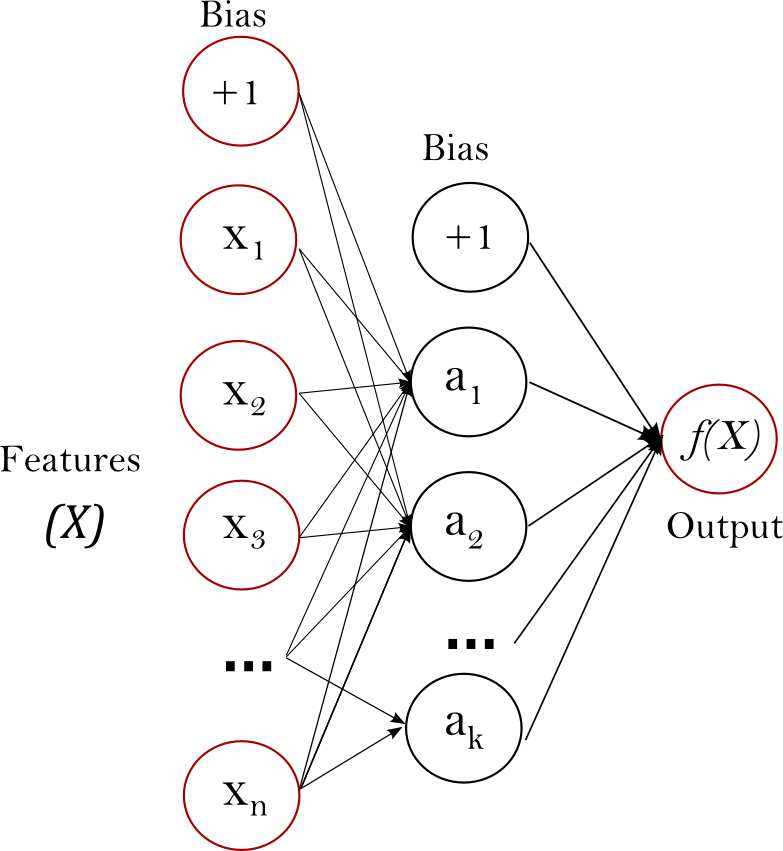
\includegraphics{multilayerperceptron_network.png}

}

\caption{Figure 1: ANN (Source: scikit-learn.org)}

\end{figure}

\hypertarget{artificial-neural-networks-1}{%
\subsection{Artificial Neural
Networks}\label{artificial-neural-networks-1}}

\begin{figure}

{\centering 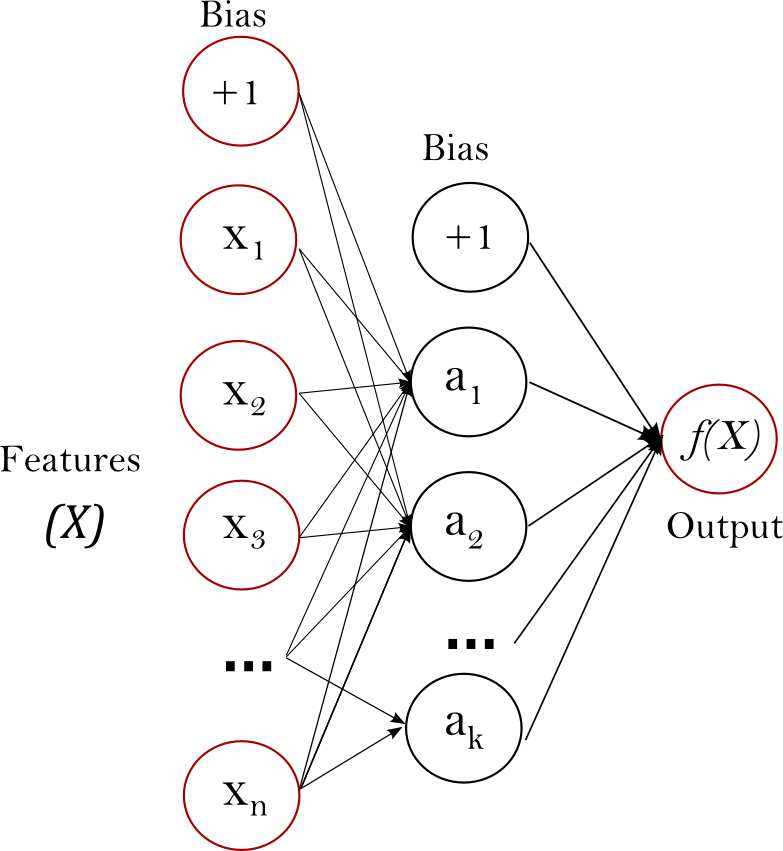
\includegraphics{multilayerperceptron_network.png}

}

\caption{Figure 1: ANN (Source: scikit-learn.org)}

\end{figure}

\begin{itemize}
\tightlist
\item
  Based on biological neural networks (neurons in a brain)
\item
  Learns function \(f(X): R^n \rightarrow R^m\)
\item
  Consists of

  \begin{itemize}
  \tightlist
  \item
    input (features) \(X\)
  \item
    hidden layers \(g(\cdots)\)
  \item
    output (target) \(y = f(X)\)
  \end{itemize}
\item
  Hidden layers can have many nodes
\item
  Neural nets can have many hidden layers (deep learning)
\end{itemize}

\begin{center}\rule{0.5\linewidth}{0.5pt}\end{center}

\hypertarget{a-single-neuron-and-a-bit-of-math}{%
\subsection{A single neuron, and a bit of
math}\label{a-single-neuron-and-a-bit-of-math}}

\begin{figure}

{\centering 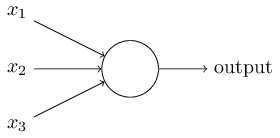
\includegraphics{perceptron.png}

}

\caption{Figure 2: Perceptron}

\end{figure}

\[\begin{equation}
y = g(w_0 + \sum_{i=1}^n w_i x_i) = g(w_0 + \mathbf{x}' \mathbf{w})
\end{equation}\]

. . .

\begin{itemize}
\tightlist
\item
  \(y\) is the output or target
\item
  \(x_i\) are the inputs or features
\item
  \(w_0\) is the bias
\item
  \(w_i\) are the weights
\end{itemize}

\begin{itemize}
\tightlist
\item
  \(g(\cdot)\) is the activation function (non-linear)
  \[\begin{equation}
  g(z) = \frac{1}{1 + e^{-z}}
  \end{equation}\]
\item
  usually a sigmoid, but there are many others
\end{itemize}

\begin{center}\rule{0.5\linewidth}{0.5pt}\end{center}

\hypertarget{training-a-neural-network}{%
\subsection{Training a Neural Network}\label{training-a-neural-network}}

Objective

\[\begin{equation}
J(\mathbf{w}) = \frac{1}{n} \sum_{i=1}^n (y_i - f(\mathbf{x}; \mathbf{w}))^2
\end{equation}\]

. . .

Optimization

\[\begin{equation}
\mathbf{w}^* = \arg \min_{\mathbf{w}} J(\mathbf{w})
\end{equation}\]

. . .

Gradient Descent

\[\begin{equation}
\mathbf{w}^{(t+1)} = \mathbf{w}^{(t)} - \eta \nabla J(\mathbf{w}^{(t)})
\end{equation}\]

\begin{center}\rule{0.5\linewidth}{0.5pt}\end{center}

\hypertarget{stochastic-gradient-descent}{%
\subsection{Stochastic Gradient
Descent}\label{stochastic-gradient-descent}}

\[\begin{equation}
\widetilde{\nabla} J(\mathbf{w}^{(t)}) = \frac{1}{B} \sum_{i=1}^B \nabla_i J(\mathbf{w}^{(t)})
\end{equation}\]

\[\begin{equation}
\mathbf{w}^{(t+1)} = \mathbf{w}^{(t)} - \eta \widetilde{\nabla} J(\mathbf{w}^{(t)})
\end{equation}\]

\begin{center}\rule{0.5\linewidth}{0.5pt}\end{center}

\hypertarget{dynamic-programming}{%
\section{Dynamic Programming}\label{dynamic-programming}}

\href{https://playground.tensorflow.org/}{Preview}

\begin{center}\rule{0.5\linewidth}{0.5pt}\end{center}

\hypertarget{the-endogenous-grid-method-by-carroll-2006}{%
\subsubsection{The Endogenous Grid Method by Carroll
{[}2006{]}}\label{the-endogenous-grid-method-by-carroll-2006}}

\begin{itemize}
\tightlist
\item
  Simple

  \begin{itemize}
  \tightlist
  \item
    Inverted Euler equation
  \end{itemize}
\item
  Fast

  \begin{itemize}
  \tightlist
  \item
    No root-finding or optimization required
  \end{itemize}
\item
  Efficient

  \begin{itemize}
  \tightlist
  \item
    Finds exact solution at each gridpoint
  \end{itemize}
\end{itemize}

\begin{center}\rule{0.5\linewidth}{0.5pt}\end{center}

\hypertarget{limitations-of-egm}{%
\subsubsection{Limitations of EGM}\label{limitations-of-egm}}

\begin{itemize}
\tightlist
\item
  \textbf{One-dimensional} problems/subproblems (nested)

  \begin{itemize}
  \tightlist
  \item
    (GEGM) Barillas and Fernández-Villaverde {[}2007{]}
  \item
    (NEGM) Druedahl {[}2021{]}
  \end{itemize}
\item
  Can result in \textbf{non-rectangular grids}

  \begin{itemize}
  \tightlist
  \item
    (Curvilinear) White {[}2015{]}
  \item
    (Triangular) Ludwig and Schön {[}2018{]}
  \end{itemize}
\item
  \textbf{Non-convexities} can be problematic

  \begin{itemize}
  \tightlist
  \item
    (DCEGM) Iskhakov, Jørgensen, Rust, Schjerning {[}2017{]}
  \item
    (G2EGM) Druedahl and Jorgensen {[}2017{]}
  \end{itemize}
\end{itemize}

\begin{center}\rule{0.5\linewidth}{0.5pt}\end{center}

\hypertarget{egmn}{%
\subsubsection{EGMn}\label{egmn}}

\begin{itemize}
\tightlist
\item
  \textbf{Insight}: Problems in which agent makes several
  \textbf{simultaneous choices} can be decomposed into \textbf{sequence
  of problems}
\item
  \textbf{Problem}: Rectilinear exogenous grid results in
  \textbf{unstructured} endogenous grid
\item
  \textbf{Contribution}: Using machine learning (GPR) to
  \textbf{interpolate} on unstructured grids
\end{itemize}

\begin{center}\rule{0.5\linewidth}{0.5pt}\end{center}

\hypertarget{the-sequential-endogenous-grid-method}{%
\subsubsection{The Sequential Endogenous Grid
Method}\label{the-sequential-endogenous-grid-method}}

\begin{itemize}
\tightlist
\item
  \textbf{Simple, Fast, Efficient}

  \begin{itemize}
  \tightlist
  \item
    Inherits properties of EGM
  \end{itemize}
\item
  \textbf{Multi-dimensional}

  \begin{itemize}
  \tightlist
  \item
    Can be used for problems with multiple state variables and controls
  \end{itemize}
\item
  \textbf{Cutting-edge}

  \begin{itemize}
  \tightlist
  \item
    Interpolation approach using a Gaussian Process Regression
  \end{itemize}
\end{itemize}

\begin{center}\rule{0.5\linewidth}{0.5pt}\end{center}

\hypertarget{consumption---labor---portfolio-choice}{%
\subsubsection{Consumption - Labor - Portfolio
Choice}\label{consumption---labor---portfolio-choice}}

Agent maximizes PDV of lifetime utility as in Bodie, Merton, and
Samuelson {[}1992{]}

\[\begin{equation}
\VFunc_0(\BLev_0, \tShkEmp_0) = \max_{\CLev_{t}, \Leisure_{t}, \riskyshare_{t}} \Ex_{t} \left[ \sum_{t = 0}^{T} \DiscFac^{t} \utilFunc(\CLev_{t}, \Leisure_{t})  \right]
\end{equation}\]

where

\[\begin{equation}
\begin{split}
    \MLev_{t} & = \BLev_{t} + \PGro_{t} \tShkEmp_{t} (1 - \Leisure_{t}) \\
    \Rport_{t+1} & = \Rfree + (\Risky_{t+1} - \Rfree)
    \riskyshare_{t} \\
    \BLev_{t+1} & = (\MLev_{t} - \CLev_{t}) \Rport_{t+1}
  \end{split}
\end{equation}\]

\begin{center}\rule{0.5\linewidth}{0.5pt}\end{center}

Recursive Bellman equation in normalized form:

\[\begin{equation}
\begin{split}
    \vFunc_{t}(\bRat_{t}, \tShkEmp_{t}) & = \max_{\{\cRat_{t},
      \leisure_{t}, \riskyshare_{t}\}} \utilFunc(\cRat_{t}, \leisure_{t}) +
    \DiscFac \Ex_{t} \left[ \PGro_{t+1}^{1-\CRRA}
      \vFunc_{t+1} (\bRat_{t+1},
      \tShkEmp_{t+1}) \right] \\
    \labor_{t} & = 1 - \leisure_{t} \\
    \mRat_{t} & = \bRat_{t} + \tShkEmp_{t} \wage \labor_{t} \\
    \aRat_{t} & = \mRat_{t} - \cRat_{t} \\
    \Rport_{t+1} & = \Rfree + (\Risky_{t+1} - \Rfree)
    \riskyshare_{t} \\
    \bRat_{t+1} & = \aRat_{t} \Rport_{t+1} / \PGro_{t+1}
  \end{split}
\end{equation}\]

where

\[\begin{equation}
  \utilFunc(\CLev, \Leisure) = \util(\CLev) + \h(\Leisure) = \frac{C^{1-\CRRA}}{1-\CRRA} + \labShare^{1-\CRRA} \frac{\Leisure^{1-\leiShare}}{1-\leiShare}
\end{equation}\]

\begin{center}\rule{0.5\linewidth}{0.5pt}\end{center}

\hypertarget{breaking-up-the-problem-into-sequences}{%
\subsubsection{Breaking up the problem into
sequences}\label{breaking-up-the-problem-into-sequences}}

Starting from the beginning of the period, we can define the
labor-leisure problem as

\[\begin{equation}
\begin{split}
    \vFunc_{t}(\bRat_{t}, \tShkEmp_{t}) & = \max_{ \leisure_{t}}
    \h(\leisure_{t}) + \vOpt_{t} (\mRat_{t}) \\
    & \text{s.t.} \\
    0 & \leq \leisure_{t} \leq 1 \\
    \labor_{t} & = 1 - \leisure_{t} \\
    \mRat_{t} & = \bRat_{t} + \tShkEmp_{t} \wage \labor_{t}.
  \end{split}
\end{equation}\]

\begin{center}\rule{0.5\linewidth}{0.5pt}\end{center}

\hypertarget{breaking-up-the-problem-into-sequences-1}{%
\subsubsection{Breaking up the problem into
sequences}\label{breaking-up-the-problem-into-sequences-1}}

The pure consumption-saving problem is then

\[\begin{equation}
\begin{split}
    \vOpt_{t}(\mRat_{t}) & = \max_{\cRat_{t}} \util(\cRat_{t}) + \DiscFac\vEnd_{t}(\aRat_{t}) \\
    & \text{s.t.} \\
    0 & \leq \cRat_{t} \leq \mRat_{t} \\
    \aRat_{t} & = \mRat_{t} - \cRat_{t}.
  \end{split}
\end{equation}\]

\begin{center}\rule{0.5\linewidth}{0.5pt}\end{center}

\hypertarget{breaking-up-the-problem-into-sequences-2}{%
\subsubsection{Breaking up the problem into
sequences}\label{breaking-up-the-problem-into-sequences-2}}

Finally, the risky portfolio problem is

\[\begin{equation}
\begin{split}
    \vEnd_{t}(\aRat_{t}) & = \max_{\riskyshare_{t}}
    \Ex_{t} \left[ \PGro_{t+1}^{1-\CRRA}
      \vFunc_{t+1}(\bRat_{t+1},
      \tShkEmp_{t+1}) \right] \\
    & \text{s.t.} \\
    0 & \leq \riskyshare_{t} \leq 1 \\
    \Rport_{t+1} & = \Rfree + (\Risky_{t+1} - \Rfree)
    \riskyshare_{t} \\
    \bRat_{t+1} & = \aRat_{t} \Rport_{t+1} / \PGro_{t+1}.
  \end{split}
\end{equation}\]

\begin{center}\rule{0.5\linewidth}{0.5pt}\end{center}

\hypertarget{solving-consumption-saving-via-egm}{%
\subsubsection{Solving Consumption-Saving via
EGM}\label{solving-consumption-saving-via-egm}}

We can condense the consumption-saving problem into a single equation:

\[\begin{equation}
\vOpt_{t}(\mRat_{t}) = \max_{\cRat_{t}} \util(\cRat_{t}) +
  \DiscFac \vEnd_{t}(\mRat_{t}-\cRat_{t})
\end{equation}\]

Interior solution must satisfy the Euler equation:

\[\begin{equation}
\utilFunc'(\cRat_t) = \DiscFac \vEnd_{t}'(\mRat_{t} - \cRat_{t}) = \DiscFac
  \vEnd_{t}'(\aRat_{t})
\end{equation}\]

EGM consists of inverting the Euler equation to find the consumption
function:

\[\begin{equation}
\cEndFunc_{t}(\aMat) = \utilFunc'^{-1}\left( \DiscFac \vEnd_{t}'(\aMat)
  \right)
\end{equation}\]

\begin{center}\rule{0.5\linewidth}{0.5pt}\end{center}

Then using budget contraint we obtain endogenous grid:

\[\begin{equation}
  \mEndFunc_{t}(\aMat) = \cEndFunc_{t}(\aMat) + \aMat.
\end{equation}\]

. . .

Using points \([\mEndFunc_t]\) and \([\cEndFunc_t]\) we can build a
linear interpolator \(\cRat_t(\mRat)\). The constraint is handled by
exogenous grid \(\aMat \ge \underline{\aRat}\) and we can add an anchor
point \(\cRat_t(\mRat = 0) = 0\) for the linear interpolator to complete
our solution.

\begin{center}\rule{0.5\linewidth}{0.5pt}\end{center}

\hypertarget{solving-labor-leisure-egm-again}{%
\subsubsection{Solving Labor-Leisure (EGM,
Again)}\label{solving-labor-leisure-egm-again}}

We can condense the labor-leisure problem into a single equation:

\[\begin{equation}
\vFunc_{t}(\bRat_{t}, \tShkEmp_{t}) = \max_{ \leisure_{t}}
  \h(\leisure_{t}) + \vOpt_{t}(\bRat_{t} +
  \tShkEmp_{t} \wage (1-\leisure_{t}))
\end{equation}\]

. . .

Interior solution must satisfy the first-order condition:

\[\begin{equation}
\h'(\leisure_{t}) = \vOpt_{t}'(\mRat_{t}) \wage \tShkEmp_{t}
\end{equation}\]

. . .

EGM consists of inverting the first-order condition to find leisure
function:

\[\begin{equation}
\zEndFunc_{t}(\mMat, \tShkMat) = \h'^{-1}\left(
  \vOpt_{t}'(\mMat) \wage \tShkMat \right)
\end{equation}\]

\begin{center}\rule{0.5\linewidth}{0.5pt}\end{center}

Using market resources condition we obtain endogenous grid:

\[\bEndFunc_{t}(\mMat, \tShkMat) = \mMat -
  \tShkMat\wage(1-\zEndFunc_{t}(\mMat, \tShkMat))\]

. . .

So we construct \(\leisure_t([\bEndFunc_t], \tShkMat)\). Actual leisure
function is bounded between 0 and 1:

\[\begin{equation}
\hat{\leisure}_{t}(\bRat, \tShkEmp) = \max \left[ \min \left[ \leisure_{t}(\bRat, \tShkEmp), 1 \right], 0 \right]
\end{equation}\]

\begin{center}\rule{0.5\linewidth}{0.5pt}\end{center}

\hypertarget{pretty-simple-right}{%
\subsubsection{Pretty Simple, Right?}\label{pretty-simple-right}}

What is the \textbf{problem}?

. . .

Exogenous Rectangular Grid

Endogenous Curvilinear Grid

. . .

One solution: Curvilinear Interpolation by White {[}2015{]}

\begin{center}\rule{0.5\linewidth}{0.5pt}\end{center}

\hypertarget{warped-grid-interpolation}{%
\subsubsection{Warped Grid
Interpolation}\label{warped-grid-interpolation}}

\begin{itemize}
\tightlist
\item
  Our solution: \textbf{Warped Grid Interpolation} (simpler, faster,
  more details on paper)
\end{itemize}

\includesvg{figures/WarpedInterpolation.svg}

\begin{center}\rule{0.5\linewidth}{0.5pt}\end{center}

\hypertarget{a-more-complex-problem}{%
\subsubsection{A more complex problem}\label{a-more-complex-problem}}

Consumption - Pension Deposit Problem as in \textbf{Druedahl and
Jorgensen {[}2017{]}}

\[\begin{equation}
\begin{split}
    \vFunc_{t}(\mRat_{t}, \nRat_{t}) & = \max_{\cRat_{t}, \dRat_{t}} \util(\cRat_{t}) + \DiscFac \Ex_{t} \left[ \PGro_{t+1}^{1-\CRRA} \vFunc_{t+1}(\mRat_{t+1}, \nRat_{t+1}) \right] \\
    & \text{s.t.} \quad \cRat_{t} \ge 0, \quad \dRat_{t} \ge 0 \\
    \aRat_{t} & = \mRat_{t} - \cRat_{t} - \dRat_{t} \\
    \bRat_{t} & = \nRat_{t} + \dRat_{t} + g(\dRat_{t}) \\
    \mRat_{t+1} & = \aRat_{t} \Rfree / \PGro_{t+1}  + \tShkEmp_{t+1} \\
    \nRat_{t+1} & = \bRat_{t} \Risky_{t+1}  / \PGro_{t+1}
  \end{split}
\end{equation}\]

where

\[\begin{equation}
  \uFunc(\cRat) = \frac{\cRat^{1-\CRRA}}{1-\CRRA} \qquad \text{and} \qquad \gFunc(\dRat) = \xFer \log(1+\dRat).
\end{equation}\]

is a tax-advantaged premium on pension contributions.

\begin{center}\rule{0.5\linewidth}{0.5pt}\end{center}

\hypertarget{g2egm-from-druedahl-and-jorgensen-2017}{%
\subsubsection{G2EGM from Druedahl and Jorgensen
{[}2017{]}}\label{g2egm-from-druedahl-and-jorgensen-2017}}

\begin{itemize}
\tightlist
\item
  If we try to use EGM:

  \begin{itemize}
  \tightlist
  \item
    2 first order conditions
  \item
    difficult to handle multiple constraints
  \item
    requires local triangulation interpolation
  \end{itemize}
\end{itemize}

\begin{center}\rule{0.5\linewidth}{0.5pt}\end{center}

\hypertarget{breaking-up-the-problem-makes-it-easier-to-solve}{%
\subsubsection{Breaking up the problem makes it easier to
solve}\label{breaking-up-the-problem-makes-it-easier-to-solve}}

Consider the problem of a consumer who chooses how much to put into a
pension account:

\[\begin{equation}
\begin{split}
    \vFunc_{t}(\mRat_{t}, \nRat_{t}) & = \max_{\dRat_{t}} \vOpt_{t}(\lRat_{t}, \bRat_{t}) \\
    & \text{s.t.}  \quad \dRat_{t} \ge 0 \\
    \lRat_{t} & = \mRat_{t} - \dRat_{t} \\
    \bRat_{t} & = \nRat_{t} + \dRat_{t} + g(\dRat_{t})
  \end{split}
\end{equation}\]

. . .

After, the consumer chooses how much to consume out of liquid savings:

\[\begin{equation}
\begin{split}
    \vOpt_{t}(\lRat_{t}, \bRat_{t}) & = \max_{\cRat_{t}} \util(\cRat_{t}) + \DiscFac \wFunc_{t}(\aRat_{t}, \bRat_{t})  \\
    & \text{s.t.} \quad \cRat_{t} \ge 0 \\
    \aRat_{t} & = \lRat_{t} - \cRat_{t}
  \end{split}
\end{equation}\]

\begin{center}\rule{0.5\linewidth}{0.5pt}\end{center}

\hypertarget{solving-the-pension-problem}{%
\subsubsection{Solving the pension
problem}\label{solving-the-pension-problem}}

The pension problem, more compactly

\[\begin{equation}
\vFunc_{t}(\mRat_{t}, \nRat_{t}) = \max_{\dRat_{t}}
  \vOpt_{t}(\mRat_{t} - \dRat_{t}, \nRat_{t} + \dRat_{t} + \gFunc(\dRat_{t}))
\end{equation}\]

. . .

Interior solution must satisfy the first-order condition:

\[\begin{equation}
\gFunc'(\dRat_{t}) = \frac{\vOpt_{t}^{\lRat}(\lRat_{t},
    \bRat_{t})}{\vOpt_{t}^{\bRat}(\lRat_{t}, \bRat_{t})} - 1
\end{equation}\]

. . .

Inverting, we can obtain the optimal choice of \(\dRat_{t}\):

\[\begin{equation}
\dEndFunc_{t}(\lRat_{t}, \bRat_{t}) = \gFunc'^{-1}\left(
  \frac{\vOpt_{t}^{\lRat}(\lRat_{t},
    \bRat_{t})}{\vOpt_{t}^{\bRat}(\lRat_{t},
    \bRat_{t})} - 1 \right)
\end{equation}\]

. . .

Using resource constraints we obtain endogenous grids:

\[\begin{equation}
  \nEndFunc_{t}(\lRat_{t}, \bRat_{t}) = \bRat_{t} -
  \dEndFunc_{t}(\lRat_{t}, \bRat_{t}) - \gFunc(\dEndFunc_{t}(\lRat_{t},
    \bRat_{t})) \\
  \mEndFunc_{t}(\lRat_{t}, \bRat_{t}) = \lRat_{t} +
  \dEndFunc_{t}(\lRat_{t}, \bRat_{t})
\end{equation}\]

\begin{center}\rule{0.5\linewidth}{0.5pt}\end{center}

\hypertarget{unstructured-grids}{%
\subsubsection{Unstructured Grids}\label{unstructured-grids}}

Problem: \textbf{Rectilinear} exogenous grid results in
\textbf{unstructured} endogenous grid

Exogenous Rectangular Grid

Endogenous Unstructured Grid

How do we \textbf{interpolate} on this grid?

\begin{center}\rule{0.5\linewidth}{0.5pt}\end{center}

\hypertarget{gaussian-process-regression}{%
\subsubsection{Gaussian Process
Regression}\label{gaussian-process-regression}}

A Gaussian Process is a probability distribution over functions

\[\begin{equation}
\begin{gathered}
    \mathbf{X} \sim \mathcal{N}(\mathbf{\mu}, \mathbf{\Sigma}) \quad \text{s.t.} \quad x_i \sim \mathcal{N}(\mu_i, \sigma_{ii}) \\
    \text{and} \quad  \sigma_{ij} = \Ex[(x_i - \mu_i)(x_j - \mu_j)] \quad \forall i,j \in \{1, \ldots, n\}.
  \end{gathered}
\end{equation}\]

where

\[\begin{equation}
\mathbf{X} = \begin{bmatrix}
    x_1    \\
    x_2    \\
    \vdots \\
    x_n
  \end{bmatrix}
  \quad
  \mathbf{\mu} = \begin{bmatrix}
    \mu_1  \\
    \mu_2  \\
    \vdots \\
    \mu_n
  \end{bmatrix}
  \quad
  \mathbf{\Sigma} = \begin{bmatrix}
    \sigma_{11} & \sigma_{12} & \cdots & \sigma_{1n} \\
    \sigma_{21} & \sigma_{22} & \cdots & \sigma_{2n} \\
    \vdots      & \vdots      & \ddots & \vdots      \\
    \sigma_{n1} & \sigma_{n2} & \cdots & \sigma_{nn}
  \end{bmatrix}.
\end{equation}\]

A Gaussian Process Regression is used to find the function that best
fits a set of data points

\[\begin{equation}
\mathbb{P}(\mathbf{f} | \mathbf{X}) = \mathcal{N}(\mathbf{f} | \mathbf{m}, \mathbf{K})
\end{equation}\]

We use standard covariance function, exploring alternatives is an active
area of research

\[\begin{equation}
k(\mathbf{x}_i, \mathbf{x}_j) = \sigma^2_f \exp\left(-\frac{1}{2l^2} (\mathbf{x}_i - \mathbf{x}_j)' (\mathbf{x}_i - \mathbf{x}_j)\right).
\end{equation}\]

\begin{center}\rule{0.5\linewidth}{0.5pt}\end{center}

\hypertarget{an-example}{%
\subsubsection{An example}\label{an-example}}

Consider the true function \(f(x) = x \cos(1.5x)\) sampled at random
points

\begin{figure}

{\centering \includesvg{figures/GPR_True_Function.svg}

}

\caption{True Function}

\end{figure}

\begin{center}\rule{0.5\linewidth}{0.5pt}\end{center}

\hypertarget{an-example-1}{%
\subsubsection{An Example}\label{an-example-1}}

A random sample of the GP posterior distribution of functions

\begin{figure}

{\centering \includesvg{figures/GPR_Posterior_Sample.svg}

}

\caption{Posterior Sample}

\end{figure}

\begin{center}\rule{0.5\linewidth}{0.5pt}\end{center}

\hypertarget{an-example-2}{%
\subsubsection{An Example}\label{an-example-2}}

Gaussian Process Regression finds the function that best fits the data

\begin{figure}

{\centering \includesvg{figures/GaussianProcessRegression.svg}

}

\caption{Alt text}

\end{figure}

\begin{itemize}
\tightlist
\item
  \textbf{Gaussian Process Regression} gives us

  \begin{itemize}
  \tightlist
  \item
    \textbf{Mean} function of the posterior distribution
  \item
    \textbf{Uncertainty quantification} of the mean function
  \item
    Can be useful to predict ex-post where we might need \textbf{more
    points}
  \end{itemize}
\end{itemize}

\begin{center}\rule{0.5\linewidth}{0.5pt}\end{center}

\hypertarget{back-to-the-model}{%
\subsubsection{Back to the model}\label{back-to-the-model}}

Second Stage Pension Endogenous Grid

\includesvg{figures/2ndStagePensionEndogenousGrid.svg}

\begin{center}\rule{0.5\linewidth}{0.5pt}\end{center}

\hypertarget{some-results}{%
\subsubsection{Some Results}\label{some-results}}

Consumption Function

Deposit Function

\begin{center}\rule{0.5\linewidth}{0.5pt}\end{center}

\hypertarget{conditions-for-using-sequential-egm}{%
\subsubsection{Conditions for using Sequential
EGM}\label{conditions-for-using-sequential-egm}}

\begin{itemize}
\tightlist
\item
  Model must be

  \begin{itemize}
  \tightlist
  \item
    concave
  \item
    differentiable
  \item
    continuous
  \item
    separable
  \end{itemize}
\end{itemize}

Need an \textbf{additional} function to exploit \textbf{invertibility}

. . .

Examples in this paper:

\begin{itemize}
\tightlist
\item
  Separable utility function

  \begin{itemize}
  \tightlist
  \item
    \(\uFunc(\cRat, \leisure) = \uFunc(\cRat) + \h(\leisure)\)
  \end{itemize}
\item
  Continuous and differentiable transition

  \begin{itemize}
  \tightlist
  \item
    \(\bRat_{t} = \nRat_{t} + \dRat_{t} + g(\dRat_{t})\)
  \end{itemize}
\end{itemize}

\begin{center}\rule{0.5\linewidth}{0.5pt}\end{center}

\hypertarget{thank-you}{%
\subsubsection{Thank you!}\label{thank-you}}

\href{https://github.com/econ-ark/HARK}{\texttt{engine:\ github.com/econ-ark/HARK}}

\href{https://github.com/alanlujan91/SequentialEGM}{\texttt{code:\ github.com/alanlujan91/SequentialEGM}}

\href{https://alanlujan91.github.io/SequentialEGM/egmn}{\texttt{website:\ alanlujan91.github.io/SequentialEGM/egmn}}



\end{document}
